\documentclass[a4paper,12pt]{article}
\usepackage{hyperref}
\usepackage{graphicx}
\usepackage{listings}
\usepackage{pdfpages}
\usepackage{color}
\lstset{breaklines=true}
\lstset{basicstyle=\small\ttfamily}
\lstset{columns=fixed}
\definecolor{Brown}{cmyk}{0,0.81,1,0.60}
\definecolor{OliveGreen}{cmyk}{0.64,0,0.95,0.40}
\definecolor{CadetBlue}{cmyk}{0.62,0.57,0.23,0}
\lstset{language=Python,
  keywordstyle=\ttfamily\color{OliveGreen},
  identifierstyle=\ttfamily\color{CadetBlue}\bfseries,
  commentstyle=\color{Brown},
  stringstyle=\ttfamily,
  showstringspaces=true}

\title{A real time train information and prediction system for the London Underground --- progress report}
\author{Murray Colpman --- Supervisor: Nick Gibbins}
\begin{document}
\begin{titlepage}
  \begin{center}
    \textsc{\Large Electronics and Computer Science}\\
    \textsc{\Large Faculty of Physical Sciences and Engineering}\\
    \textsc{\Large University of Southampton}\\[1.5cm]
    \textsc{\Large Murray Colpman}\\
    \textsc{\Large \today}\\[1.5cm]
    \textsc{\LARGE A real time train information and prediction system for the London Underground}\\[1.5cm]
    \textsc{\large Project supervisor: Nick Gibbins}\\
    \textsc{\large Second examiner: Iain McNally}\\[1.5cm]
    \textsc{\large A project progress report submitted for the award of}\\
    \textsc{\large MEng Computer Science --- 4443}
  \end{center}
\end{titlepage}

\section*{Abstract}

The London Underground currently lacks publicly-available software allowing its
users to track individual trains through the system. This project aims to
resolve this by creating a system to allow the user to view a list of trains
due to depart each station along with ones already departed, and to allow the
user to select a train to view its course throughout the system. So far,
background research has been performed, the overall design of the system has
been decided and a basic implementation of a tool to gather the data that will
be necessary to reconstruct the timetable has been produced, to run over the
coming months. Most of the implementation is still to be performed, including
producing an algorithm to reconstruct the timetable based on the real train
movements over a number of days, and a web interface to navigate around the
system. The stretch goals are to produce a system to predict times based on
actual performances of trains, and to produce a map of track codes (signalling
blocks that trains can occupy) based on the gathered data to further improve
predictions.

\pagebreak

\tableofcontents

\pagebreak

\section*{Statement of Originality}

This is all my own work except where explicitly indicated otherwise, and all
sources have been correctly acknowledged.

\pagebreak

\section{Introduction}

The London Underground is a source of great interest for rail enthusiasts. With
its own rich history, there are occasional heritage operations such as the
recent Steam on the Met events organised by the London Transport Museum. Stock
withdrawal causes great interest in its own right, for example the desire to
ride on the last train of particular stock, or to ensure that you have ridden
on all trains before they are withdrawn. Finally, unique activities like the
Tube Challenge (visiting every London Underground station arriving or departing
by train in one day) also offer interest.

All of these tasks are currently hindered by the lack of a publicly-available
information system that allows the user to track trains through the network,
and yet the data required to create one is more or less available. This project
aims to create such a system, allowing the user to view the arrivals and
departures in the near past, present and the future for a given station, and
also to track a given train through the system.

Such a system will be primarily designed for rail enthusiasts. But as a
byproduct of producing the system, data will be collected which will allow a
few inferences to be made about the system. A small number of these will
additionally be explored.

\section{Project Description and Background}

\subsection{Realtime Trains --- an information system for the national railway
network}

Rail enthusiasts make use of a website called Realtime Trains. For the National
Rail network, on which the vast majority of heavy rail services in Great
Britain run, this website makes use of open data mainly from four sources
provided by Network Rail (the public body that owns and maintains the
infrastructure and operates signalling equipment for nearly all of the
network)\cite{RTTData}:

\begin{itemize}
  \item TRUST, providing push data about trains passing certain timing points
    (mostly stations and junctions)
  \item TD, push data providing the train describer berth (which corresponds to
    a signalling section) that a given train is occupying --- cross-referenced
    with TRUST data to give more accurate predictions and platform alterations
  \item Schedule, pull data providing timetables for passenger and freight
    trains including changes to usual services (for engineering works, for
    example)
  \item VSTP, push data providing very short notice alterations to schedules
\end{itemize}

Realtime Trains uses these data sources to give views for the general public to
let people know where their train is, and to predict arrival times. It also has
a detailed view, allowing enthusiasts to see non-passenger trains, trains not
booked to stop at the station, detailed information about the routes trains are
booked to take (and actually take), and more detailed timing points. This can
be used by enthusiasts to track the position of a train they're interested in,
or just to see if any interesting trains are passing through a station.

\subsection{Adapting the concept to the London Underground}

The London Underground, despite having a few areas of overlapping operation, is
not generally a part of the National Rail network, and so Realtime Trains does
not allow you to view information for the vast majority of its 270 stations.

Although the London Underground has an information system geared towards the
general public, there is currently no publicly-available software to track
individual trains through the system, nor is there a way to view the timetable
(both planned and predicted) from each station more than a few trains in
advance. Only ``live departure board'' style sites are available, showing for
each station when the next trains are due.

Such a tracking system would not only be useful for rail enthusiasts, for
example trying to follow a delayed steam service around the network or to
follow a particular train of interest, but would also be very useful for making
a variety of inferences about the network.

The main source of open data comes from a system called TrackerNet. TrackerNet
is a pull-based system, so a request must be made by the client every time new
data is desired. Data is requested over HTTP and returned in an XML format. To
prevent flooding, this data is cached for around thirty seconds (though in
reality, caching up to a minute is common).

There are four main endpoints available when using this data --- LineStatus
which returns overview information about the operation of each line (whether
there is disruption or closures), StationStatus which gives similar information
about stations, PredictionSummary which gives basic train prediction
information on a per-line basis, and PredictionDetailed which gives more
detailed train prediction information. This is requested on a per-station and
per-line basis\cite{TrackerNetSpec}. Therefore, one request per station desired
for each line is required per half minute. When this report refers to
TrackerNet, unless otherwise stated the PredictionDetailed endpoint is meant.

This data contains an attribute called TrackCode, which is the most accurate
source of location data --- it represents the current signalling block in which
the train is located. However, there is no publicly-available data to represent
the location of track codes, neither geographical nor topological. The caching
of data and the fact that some track codes are quite short (less than 30
seconds apart) means that it is less than trivial to construct such a map.

There is another source of data --- the public timetable as used by the TfL
journey planner. It is stored in a format known as TransXChange, a format
developed as a national standard for storing UK bus
timetables\cite{TransXChangeSpec}. Unfortunately, this data does not receive
any supplements for engineering works or alterations to the usual timetable. It
also doesn't contain non-passenger trains, like empty workings or engineering
trains, which would be important to enthusiasts. Finally and crucially, as far
as I can tell there is no way to relate this data with the live data.

There are also PDF working timetables available\cite{TfLWTT}, which do contain
all trains and do contain IDs which can be cross-referenced with the live data
--- a set number, representing one particular train's workings throughout the
day; and a trip number, which increments each time the train terminates and
forms a new working.

\subsection{Goals and scope}

\begin{enumerate}
  \item To produce a software system to track trains throughout the London
    Underground System and store the results of past days
  \item To infer the working timetable for this data by averaging past runs
  \item To produce a web-based user interface for viewing this data per-station
    or per-train
  \item To expand the system to predict the future arrival and departure times
    of trains, including when forming new services
  \item To produce a topological map of track codes, and to use this map to
    further improve the predictions
\end{enumerate}

The main project comprises goals 1--3. Goals 4 and 5 are stretch goals.
Evaluation of the main project can be performed by testing a sample of the
produced timetable manually against the PDF and seeing how well they match.
Evaluation of goal 4 involves seeing how well the predictions match subsequent
reality. Evaluation of goal 5 is more difficult --- if a portion of a track
code map cannot be obtained, checking the map to ensure that at least the track
layout matches reality (maps of the London Underground track layout not
including signalling or track code data are commercially available from
TRACKmaps\cite{TRACKmaps5}) would be a reasonable evaluation step.

\section{Background research}

There have been a few analyses published on the state of open data on various
forms of public transport. This section is intended to summarize this state for
railways in particular, including light rail and rapid transit systems like the
London Underground.

The recent Parliamentary Office of Science and Technology
briefing\cite{POSTnote472} states that the Department for Transport currently
publishes 255 datasets, of which 244 are issued under the Open Government
licence, which is a Creative Commons-compatible open data licence. However,
there are a further 481 datasets that are not currently published --- the vast
majority. It also states that data is frequently not retained or archived in
the sector. There is also the issue of the data being usable --- data that is
hard to use, or that is of questionable quality, will not encourage as much
usage as good quality and easy to use data. Fixing these issues may be
expensive and time-consuming, so there is a trade-off involved in opening up
data. It is worth noting that one user of Transport for London's London
Underground open data, the author of Twitter bot @whensmytube, noted that it is
much more difficult to use and less useful than the equivalent data for buses
on his blog\cite{whensmytube}.

However, over-processing can also be a problem --- it has, for example, been
argued that raw data is often more useful than data pre-processed, perhaps
(intentionally or otherwise) with specific use cases in mind that sometimes
limit what can be done\cite{Robinson2009}. The wide variety of use cases of
open data should be kept in mind --- use cases for railway-related data can be
split into three broad categories\cite{Kuhn2011}: advanced search, to allow
users to search for specific attributes that may not be possible using the
operator's own website; mash-ups, which combine railway data with data from
other sources; and visualisations, for example a heat map of areas with most
delay, or a map showing where trains are physically located --- the latter of
which has been built for the London Underground using TrackerNet
data\cite{TrainTimesTube}.

Another survey, of accessibility data in particular, notes the difficulties of
relating data from multiple sources, and suggests publishing data as linked
open data to solve this\cite{Ding2014}.

There is also the issue that trains are operated commercially by multiple
companies, which causes data to be inconsistently available, or available but
not under open licences. For example, National Rail Enquiries (a part of the
Association of Train Operating Companies (ATOC), an association of all
passenger operators on the national network) until recently charged to access
their data. They now provide free access to individuals and small
organisations, but still charge a considerable fee for sites which have more
than five million usages in a four week period, meaning it is not true open
data. This data is the only source of some information on the National Rail
network such as delay causes and certain methods for train
cancellation\cite{CairnsSeminar2013}.

\section{Potential approaches (including final approach and justification)}

\subsection{Database}

A database is required to store past data, both for retrieval and for making
inferences.

There are multiple options for both the database engine and for the structure
of the database. For the database engine, the main choices are traditional
relational SQL-based databases such as MySQL, MariaDB and PostgreSQL; and
modern NoSQL databases that eschew the relational model in favour of others,
such as MongoDB which uses a document model.

Based on my prior knowledge combined with a little research, I determined that
NoSQL databases are generally more useful when storing data which is only
loosely structured or needs to be easily extensible. Since the data being
stored does not meet these criteria, I quickly decided on a relational
database.

For structuring the data in the database, there are also multiple approaches.
The most obvious approach is in a similar structure to the TrackerNet XML ---
stations have platforms which have trains in various states of approach at
different times. Trains could alternatively be linked specifically to locations
such as track codes as opposed to the requested station, but this could prove
troublesome since I have seen the occasional train in the data which had an
empty string for the track code.

There is also the possibility of tailoring the data for specific purposes ---
for example pre-calculating parts of averages of arrival times so that
relatively little database access would be needed to calculate the inferred
timetable, or even storing the same data multiple times in different structures
entirely for different purposes.

Storing data in its rawest form seems most useful, and it will
always be possible to incorporate aspects of the other ideas above should
calculations prove too slow in practice, once enough data has been collected.
However, some irrelevant, broken or not implemented data should not be saved to
the database.

Therefore, there will be three main tables:
\begin{itemize}
  \item stations --- one entry per station per line. Containing lineCode and
    code (which form a primary key), lineName and name.
  \item platforms --- one entry per station platform. Containing number, name
    and trackCode (the track code for the front of the platform), along with
    foreign keys stationLineCode and stationCode referencing stations.
  \item trains --- one entry per train per caching time, for each platform.
    Containing lcid (an ID for the leading vehicle), setNo and tripNo (which
    together form the identity of the train in the timetable), secondsTo (the
    time until the train arrives at the station), location (human-readable),
    destination (human-readable), destCode (numeric ID signifying route of
    train), trackCode, ln (line, useful for subsurface trains), whenCreated
    (when the data was created that identifies this particular location), along
    with foreign keys stationLineCode, stationCode and platformNumber
    referencing platforms.
\end{itemize}

\begin{figure}[h]
  \centering
  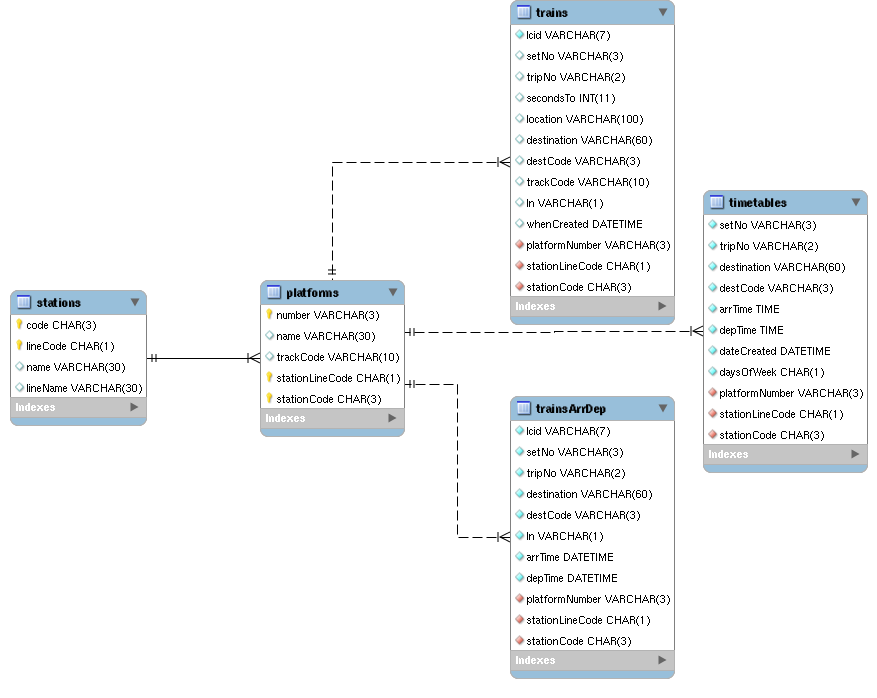
\includegraphics[width=\linewidth]{erd}
  \caption{Entity Relationship Diagram for database structure}
  \label{fig:erd}
\end{figure}

\subsection{Language choice}

The programming language in which the program is to be written is important. A
good choice in language can make a project easy to build and maintain and
increase reliability, whereas a poor choice can do just the opposite. I have
excluded obviously unsuitable languages, and languages in which I have little
experience.

Java is an obvious contender, being ubiquitous and versatile. However, it has
two important drawbacks --- it is not particularly suited for server-side web
development, and it is hard to get things done quickly, requiring a lot of
boilerplate code.

PHP is a popular choice for server-side web code, and would probably have
library support for everything that I might need to do. The main drawback is
that the design of the language is so poor that in my personal opinion too much
time is spent during development finding and fixing bugs that simply wouldn't
exist in most other languages.

Finally, Python is a mature language strongly suited to web development with a
large selection of libraries available. Getting things done is easy, but at the
expense of things like static typing which can lead to bugs or make debugging
harder. However, the design of the language is generally sound, certainly
moreso than JavaScript or PHP. It also has the issue that still not all
libraries are compatible with Python 3, which is the sensible choice for new
developments. However, despite these minor drawbacks, it is still, in my
opinion, the best language for this particular job, so I will be using it for
all server-side design.

\subsection{Client-side website}

Since this project is mostly geared towards the backend than the frontend, I
need a simple web client that requires little set up and does not do much
client-side scripting, but still looks good. For this purpose, Twitter
Bootstrap, with which I am familiar at least in passing, is a reasonable
framework to use. There are other more complex frameworks available, but since
I am not particularly familiar with client-side web development, Twitter
Bootstrap is probably the easiest option here.

As for the look of the page, the most intuitive design is to have a search page
for stations, time periods and other filters; a results page for a single
station's trains for the time period specified and filtered using the given
filters; and a page for a single train's locations (past, present and future).
No alternative designs come to mind for this, and this design matches that of
most similar sites such as Realtime Trains, Open Train Times and National Rail
Enquiries.

\begin{figure}[h]
  \centering
  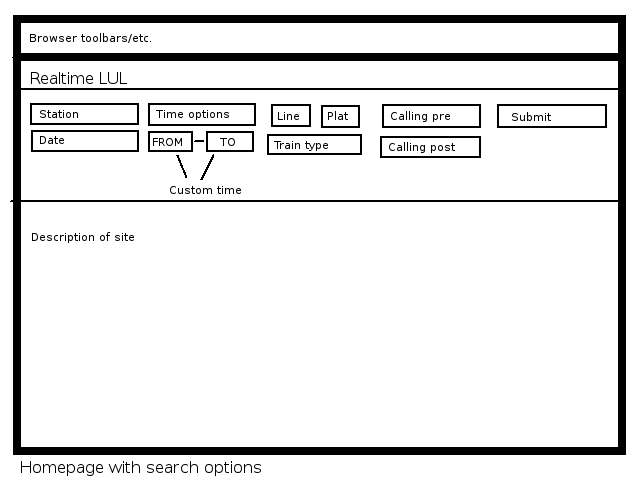
\includegraphics[width=\linewidth]{screen1}
  \caption{Diagrams of front page layout}
  \label{fig:screen1}
\end{figure}
\begin{figure}[h]
  \centering
  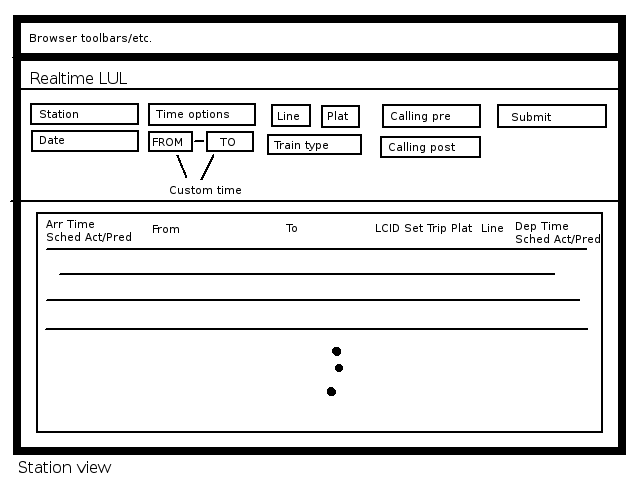
\includegraphics[width=\linewidth]{screen2}
  \caption{Diagram of station page layout}
  \label{fig:screen2}
\end{figure}
\begin{figure}[h]
  \centering
  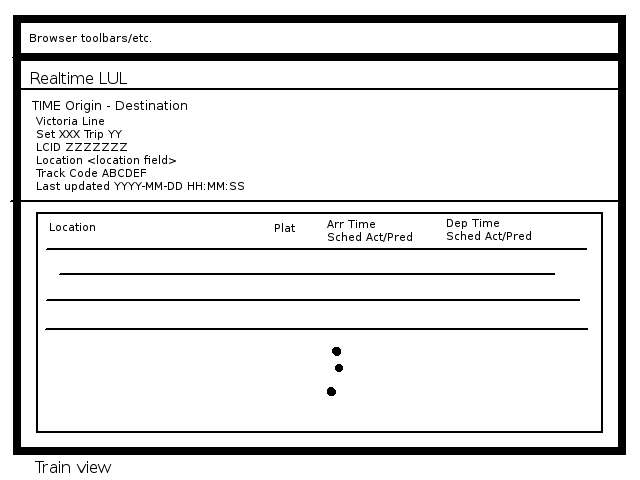
\includegraphics[width=\linewidth]{screen3}
  \caption{Diagram of train page layout}
  \label{fig:screen3}
\end{figure}

The software itself will be split up into modules. There will be a few entry
points to the software --- different scripts tying the modules together in
different ways. For example, there will be the data-gathering script, the web
server script (HTML output through a templating library along with raw JSON)
and the timetable inference tool. The modules will include a database access
module, a module to parse the TrackerNet data, and modules to handle searching
and templating. The software will be based around station, platform and train
objects, mirroring the database entries.

\section{Work to date}

I have produced an implementation of a tool to gather TrackerNet data for one
line and dump it in the database. Most of this tool is included in the
Appendix. It contains a complete implementation of a module to download and
extract data from TrackerNet, an implementation of the write functions for
database access, definitions of which stations are on which lines (not
included), a set of classes to store stations, platforms and trains, and a
script to tie all these together and use them to gather the data in a loop.

\section{Remaining work}

The database module needs to be able to read from the database. Then I can
produce another module that infers the timetable. The whole web interface needs
creating, as does the search engine. Timetable data needs to be stored, and
combined with the live data.

\section{Support required}

I do not envisage any support being required.

\section{Time management and Gantt chart}

Good time management is important in this project. So far, the project has been
more or less on schedule; although there are some aspects of design that are
not yet finalised, these require data to be gathered for the current
implementation so experiments can be run to ascertain the best methods.

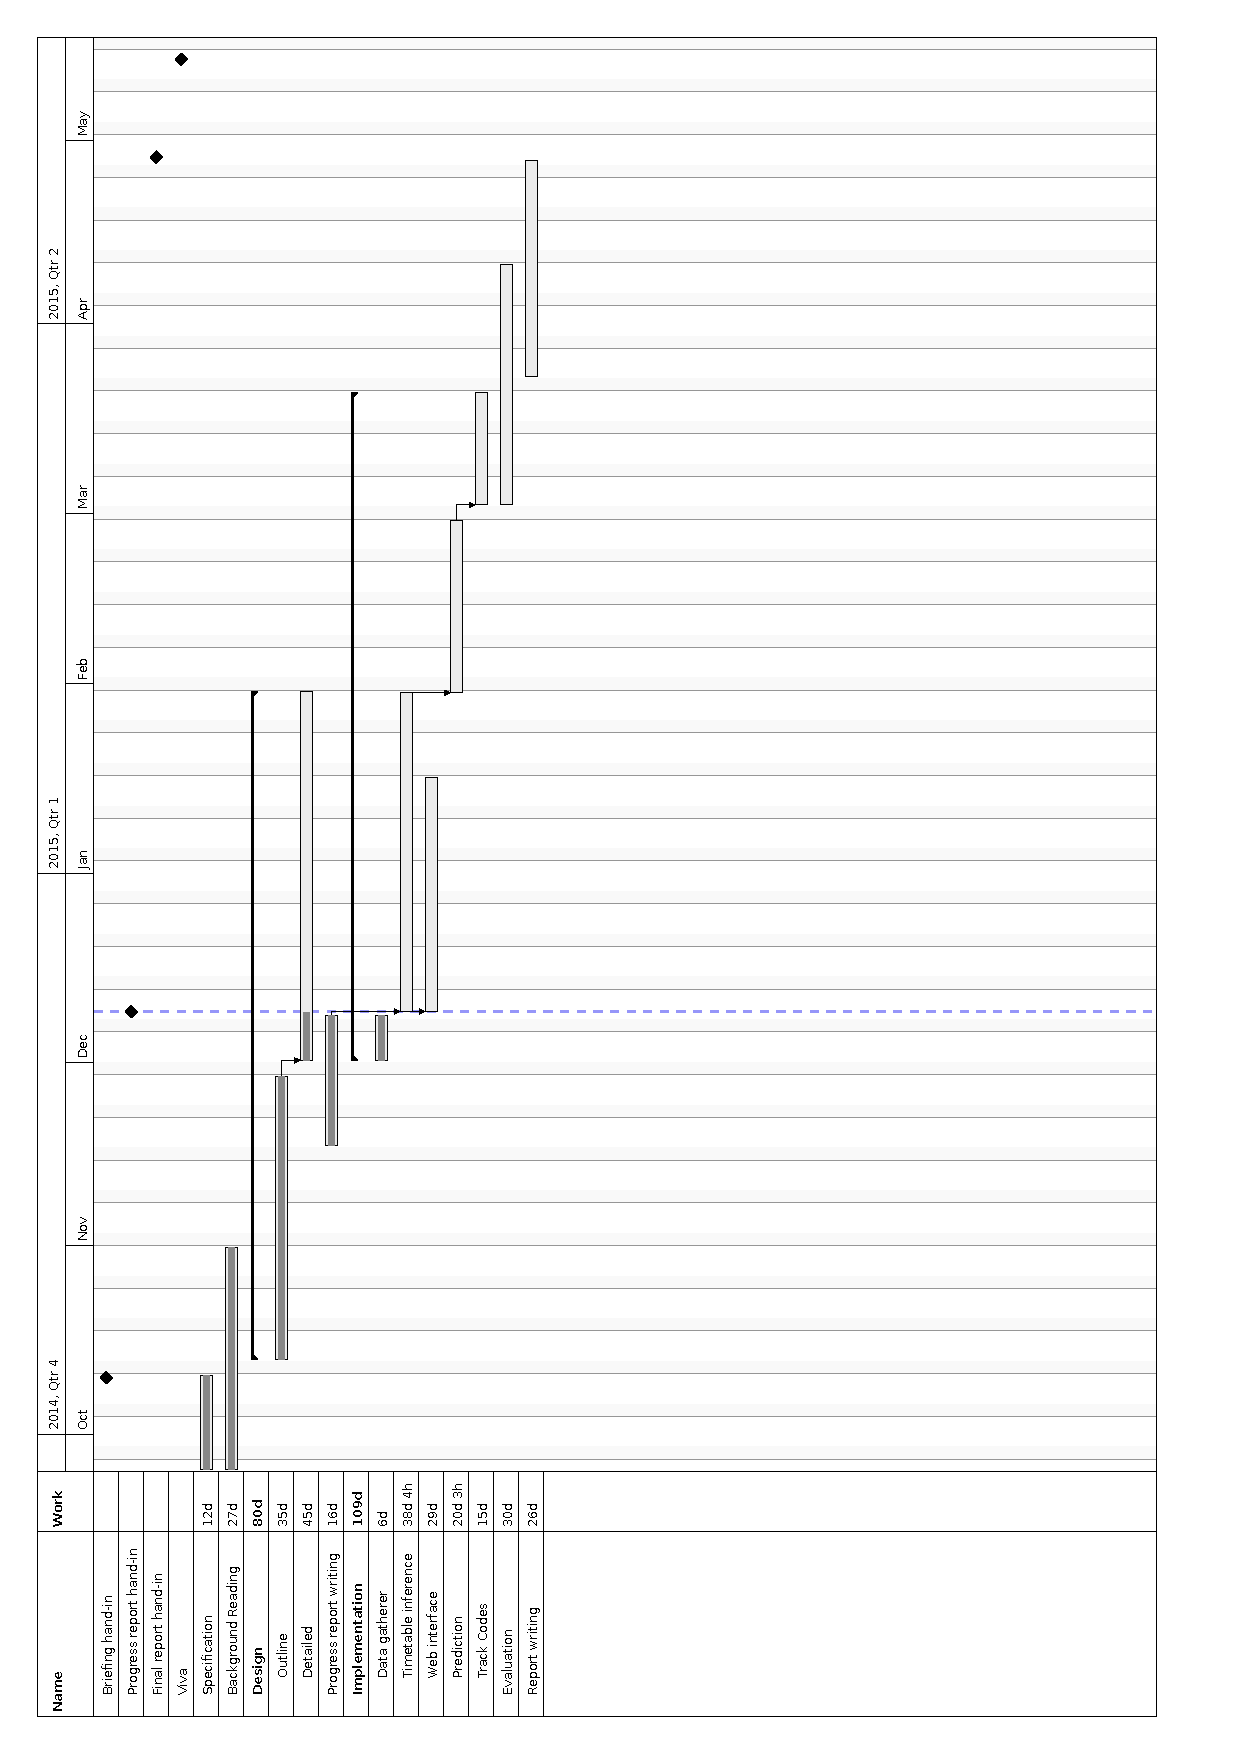
\includepdf{gantt.pdf}

\section{Conclusion}

This project has not reached any unexpected problems, and is currently on time.
The data available looks to be good enough to be likely to produce reasonable
results, and I will be continuing the implementation once I have gathered
enough data over Christmas.

\pagebreak

\section*{Appendix A --- Code Sample}

\subsection*{trackernet\_access.py}

\lstinputlisting{../code/trackernet_access.py}

\section*{Appendix B --- Archive contents}

\begin{itemize}
  \item data\_logger.py --- entry point for data logger
  \item database\_access.py --- database access module
  \item linedefs.py --- definitions of which stations are on which lines
  \item station.py --- station, platform and train classes
  \item trackernet\_access.py --- TrakerNet access and parsing module
  \item README.txt --- Readme for python setup and database installation
\end{itemize}

\bibliographystyle{acm}

\bibliography{references}

\end{document}
